\documentclass[conference]{IEEEtran}
\IEEEoverridecommandlockouts

\usepackage{amsmath,amssymb}
\usepackage{graphicx}
\graphicspath{{figures/}}
\usepackage{booktabs}
\usepackage{array}
\usepackage{subcaption}
\usepackage[none]{hyphenat}   % no hyphens at line breaks
\usepackage{url}
\usepackage{microtype}
\usepackage[hidelinks]{hyperref}
\hypersetup{pdfauthor={Abhishek Tyagi},pdftitle={Which Demonstration Mistakes Hurt Imitation Learning?},pdfsubject={CS59300 ILR Project Final Report}}
\usepackage{stfloats}
\usepackage{placeins}
\DeclareMathOperator{\clip}{clip}
\sloppy
\emergencystretch=3em

\begin{document}

\title{Which Demonstration Mistakes Hurt\\Imitation Learning?\\[0.2em]
\large A Controlled Study of Error Types in Robot Navigation}

\author{\IEEEauthorblockN{Abhishek Tyagi, Nishad Gupta, Richard Li}
\IEEEauthorblockA{CS59300 Imitation Learning for Robotics\\
Final Project Report, November 2026}}

\maketitle

\begin{abstract}
We study how specific kinds of mistakes in demonstration data change a behavior cloning (BC) policy for robot
navigation. Six flawed versions of a scripted maze driver each drive a share of the training trips with one kind
of mistake, and we score every resulting policy with paired statistical tests, not only averages. With ten
training seeds for the main comparison, three mistakes clear every test we apply, including a seed paired
permutation test after correction for six comparisons: a delayed turn at corners raises wall contact by 30
points, a missing recovery step by 14 and wall hugging by 11, and all three hold on maze routes the training data
never contained. The other three do not: wrong turns into side corridors show no collision effect at a 20\%
corrupted share, though they cost 15 points of success once every trip carries one, and a fast driving speed is a
working faster style that only hurts when mixed with the normal speed. No pair of mistakes hurts more than the
sum of its parts, yet mixing all six into one dataset hurts more than the average single mistake does. A small
classifier reads a policy's own test rollouts and names which of six mistakes trained it with 72\% accuracy
against a 17\% chance rate, and 70\% at a corruption strength it never trained on, though it cannot tell a clean
policy from a flawed one.
\end{abstract}

\begin{IEEEkeywords}
imitation learning, behavior cloning, demonstration quality, robot navigation, data corruption
\end{IEEEkeywords}

%=======================================================================
\section{Introduction}

Imitation learning assumes the demonstrator is worth imitating. In practice a demonstration set is rarely clean:
a human teleoperator turns a corner late, drifts toward a wall, takes a wrong corridor and backs out, or simply
drives faster than the policy should. Most published treatments of this problem describe demonstration quality
with one scale, from worse to better, and ask how to down weight the worse end. That framing leaves a practical
question unanswered. If only part of a dataset can be cleaned or relabeled, which kind of mistake should be
removed first?

This project asks a narrower question that can be answered by a controlled experiment:

\emph{When a fixed share of the demonstrations used to train a behavior cloning navigation policy contains one
specific kind of mistake, which kinds of mistake change the learned policy the most, and what property of a
mistake decides whether it carries over into the policy?}

We answer it by building six flawed versions of a scripted expert for a maze navigation task, each committing one
named mistake, and by holding everything else fixed: the same 500 trips, the same start and goal cells, the same
simulator seeds, the same network, the same training recipe and the same 200 test trips. Only the kind of mistake
changes in the main comparison, and the share of corrupted trips changes in a second set of runs. In total the
study trains and scores 165 policies across 26 datasets: five seeds for every dataset, and ten for clean BC and
the six errors at the main 20\% share.

Three findings survive every statistical test we apply. A delayed turn at corners raises the share of test trips
with a wall contact by 30 points, a missing recovery step by 14 points and wall hugging by 11 points. With ten
seeds per side all three clear a seed paired permutation test after correction for six comparisons, the
strictest of our checks, and all three hold on maze routes absent from the training data. Missing recovery holds
even after every error is cut to the same number of wrong training steps, which makes it the most harmful of
the six per wrong step. The remaining three mistakes show no collision effect at the main share: the two wrong
turns are flat, and a faster driving speed turns out not to be a mistake at all once the whole dataset uses it.

Three further results come out of the same policies. No pair of mistakes placed on the same trips hurts more than
the two hurt separately, while spreading all six mistakes across one dataset hurts more than the average single
mistake does. A classifier that sees only a policy's own test rollouts, never its training data, names which of
six mistakes trained that policy with 72\% accuracy against a 17\% chance rate, and 70\% when tested at a
corruption strength held out of its training. Doubling the number of policies lowered the first figure from 83\%,
so the smaller run had been optimistic. The same classifier cannot reliably tell a clean policy from a flawed one,
which marks the limit of this kind of diagnosis.

\subsection{What changed since the midterm}
The midterm reported the six single errors at one corrupted share, judged by a descriptive rule: a difference
counted when it exceeded twice the larger seed standard deviation. Six things changed after that report.

That descriptive rule became a statistical test. Each comparison now carries an exact permutation test over the
ten training runs behind it, with Holm correction across the six main errors, alongside a paired bootstrap
interval and a seed matched interval. A result counts as solid only when both intervals exclude zero and the
permutation p value survives the correction.

The main comparison was extended to ten training seeds. A review of an earlier draft pointed out that at five
seeds a seed paired test could not reach significance after correction, however large the effect; ten seeds
remove that limit, and they moved wall hugging from suggestive to established.

The corrupted share and the amount of wrong data are now varied on purpose. The same six errors were rebuilt at
50\% and 100\% of the trips, and three of them were cut down to the same number of wrong steps as a wrong turn
carries, so the dose of a mistake and the kind of mistake are no longer tangled together.

Three pairs of errors and one mixture of all six were trained and scored, and the interaction test proposed at the
midterm is now computed from resampled seeds and trip positions rather than from combined standard errors.

The diagnosis classifier that the midterm listed as a plan was built, and pushed past its first form: it is now
tested at a corruption strength held out of training, and on the harder question of telling a clean policy from a
flawed one.

An unseen route generalization check was added that the midterm did not plan for. The 200 test trips split into those whose
start and goal cells were used together in training and those that were not, which lets every finding be checked
against routes the policy never practiced.

%=======================================================================
\section{Related Work}

\subsection{Behavior cloning and compounding error}
Behavior cloning treats imitation as supervised learning from state to action, an idea that goes back to ALVINN,
which drove a vehicle from camera images through a small neural network trained on recorded human steering
\cite{pomerleau}. Its weakness is well understood. Ross and Bagnell showed that a policy trained this way sees
only the states the expert visited, so any error moves the learner into unfamiliar territory where the error
grows, and the total cost can scale with the square of the task horizon rather than linearly \cite{ross2010}.
DAgger removes that failure mode by collecting labels on the states the learner itself reaches, repeatedly
querying the expert as the policy improves, which reduces the problem to no regret online learning and recovers a
linear bound \cite{dagger}.

This line of work assumes the expert's labels are correct. It explains why unfamiliar states are dangerous, and
it offers an answer when the expert is available for more queries, yet it says nothing about what happens when
the labels themselves contain mistakes. The failure it describes and the failure we study can occur together: a
flawed label pushes the policy toward a state the expert rarely visited, and compounding error takes over from
there. We keep the learner fixed at plain BC, with no interactive querying, so that any change we measure comes
from the labels rather than from the learning rule.

\subsection{Noise injection and recovery data}
DART attacks the same covariate shift from the data collection side. It perturbs the actions the expert executes
during collection while recording the action the expert meant to take, so the demonstrations pass through states
slightly off the ideal route and show how to return to it \cite{dart}. The noise is random, carries no consistent
direction, is applied with the expert's intent still recorded, and is added to help.

Our mistakes invert each of those properties. They are structured rather than random, they are recorded as the
labels rather than corrected in the recording, and they are meant to hurt. One of our six, the missing recovery
error, is close to DART run backwards: the slip off the route is recorded, and the steps that steer back are
deleted, which removes exactly the examples DART adds. That error turns out to be one of the three our results call
solid, and the most harmful of the six per unit of wrong data.

\subsection{Measuring demonstration quality}
A second line of work measures quality rather than repairing it. The robomimic study trained the same policies on
demonstrations from human operators of different skill and found large gaps in the resulting success rates,
enough to dominate most algorithmic choices \cite{robomimic}. Belkhale et al.\ formalize demonstration quality
through two quantities, how far an action diverges from what the learner would do and how much of the state space
the transitions cover, and show that the two interact rather than adding \cite{belkhale}.

Both describe a dataset with aggregate properties, which is the right level for choosing between datasets and the
wrong level for deciding what to fix inside one. A single number for divergence cannot distinguish a demonstrator
who turns late at every corner from one who occasionally wanders into the wrong corridor, though our results show
those two leave very different policies behind. We hold the share of corrupted trips fixed in the main comparison
and change only the kind of mistake, then vary the share separately, which separates the two axes those aggregate
measures combine.

\subsection{Learning from imperfect demonstrations}
Several methods learn usable policies from demonstrations known to be imperfect. Wu et al.\ attach confidence
scores to a small labeled subset and reweight the rest through semi supervised estimation \cite{wu2019}. Sasaki
and Yamashina avoid the need for such scores, noting that a policy trained on a mixture of good and bad
demonstrations can be used to reweight its own training data over several rounds \cite{sasaki}. Brown et al.\
go further and extract a reward from ranked sub optimal demonstrations, which allows the learned policy to beat
every demonstrator it was shown \cite{trex}.

These methods treat bad data as generic sub optimality, to be discounted by a weight or a rank. None asks which
mistakes matter most, so none offers guidance on where a limited cleaning budget should go. Our results name the
three error types that would be worth filtering first, and show that the other three leave no measurable mark on
collisions at the share we studied most closely.

A related question has a long history in supervised learning, where label noise is modeled explicitly and
estimators are corrected for it \cite{natarajan}. The sequential setting differs in an important way: a wrong
action in navigation changes every state that follows it, so a corrupted demonstration damages both the labels
and the distribution of states those labels describe.

\subsection{Corruption benchmarks}
Hendrycks and Dietterich built a benchmark of named image corruptions at controlled severities and measured how
each one degrades a classifier, which turned a vague notion of fragility into a table that can be compared across
models \cite{hendrycks}. That benchmark concerns inputs at test time for a one step prediction problem.

We borrow its design, a taxonomy of named corruptions applied at a controlled share of the data, and move it to
the training demonstrations of a sequential policy, where the same corruption affects the labels and the state
distribution at once. We add what a benchmark of this kind needs to be trusted at our sample size: a correction
for multiple comparisons, intervals from two resampling schemes, and a check that each finding survives on routes
the training data never contained.

\subsection{Position of this work}
This project contributes (1) a controlled comparison of six concrete navigation mistakes across three corrupted
shares, with statistical tests behind the three findings that hold up; (2) measured interactions, sub additive for
every pair of mistakes and super additive for a mixture of all six; (3) a classifier that names the training
mistake from rollouts alone, including at a corruption strength never seen in training; and (4) evidence that the
three solid findings are not an effect of memorized routes.

%=======================================================================
\section{Preliminaries}

\subsection{Behavior cloning as supervised learning}
The state is $s=(x,y,v_x,v_y,g_x,g_y)\in\mathbb{R}^6$, holding the ball's position, its velocity and the goal,
and the action is a force $a=(f_x,f_y)\in[-1,1]^2$. An expert policy $\pi^*$ and, for each error type $k$, a
flawed policy $\tilde\pi_k$ drive trips through the maze. Dataset $D_k$ contains $N=500$ trips, of which a share
$\alpha N$ is driven by $\tilde\pi_k$ and the rest by $\pi^*$, with $\alpha\in\{0.2,0.5,1.0\}$ depending on the
run. BC fits a network $\pi_\theta$ by minimizing the squared error between its output and the recorded action,
\begin{equation}
  L(\theta)=\frac{1}{|D_k|}\sum_{(s,a)\in D_k}\big\|\pi_\theta(s)-a\big\|^2 .
  \label{eq:loss}
\end{equation}

\subsection{Why a wrong label can persist}
The minimizer of the expected squared error at a state is the mean action recorded at that state. If a share
$p_k(s)$ of the rows near $s$ come from the flawed driver, the learned policy approaches a blend of the two
drivers,
\begin{equation}
  \pi_\theta(s)\;\approx\;a^*(s)+p_k(s)\,\big(\tilde a_k(s)-a^*(s)\big).
  \label{eq:bias}
\end{equation}
Equation~\eqref{eq:bias} gives a testable prediction. A mistake transfers into the policy when its bias term
$\tilde a_k-a^*$ points the same way across many states and trips, since those contributions add. A mistake
averages out when it is rare, or when its bias term points in a different direction each time it occurs, since
those contributions cancel. Section~\ref{sec:results} checks this prediction against the mistakes that turned out
to survive every statistical test, and reports where it falls short.

The prediction depends on the squared error objective, which is what makes averaging the right behavior for the
network. Objectives that model the action distribution rather than its mean, such as energy based formulations of
BC \cite{florence}, would not blend two drivers the same way, so the ranking reported here belongs to the
standard regression form of BC rather than to imitation learning in general.

\subsection{Environment}
We use the Medium PointMaze task (version 3) from Gymnasium Robotics \cite{gymrobotics}, a descendant of the D4RL
maze tasks \cite{d4rl}. A ball of radius 0.1 moves through an $8\times8$ grid of unit cells, where walls form the
outer ring and several internal blocks, leaving 26 open cells and so 650 ordered start and goal pairs. The action
is a force rather than a velocity, so the ball carries momentum and has to brake before a corner, which is what
makes a late turn a physically meaningful mistake. A trip succeeds when the ball comes within 0.5 of the goal and
is cut off after 600 steps. We chose Medium over the smaller UMaze after a pilot run: on UMaze, BC on clean data
already reached 100\% success, which leaves no room to measure damage. Figure~\ref{fig:expert} shows a sample of
expert trips and the speed profile the controller holds along them.

\begin{figure}[tbp]
\centering
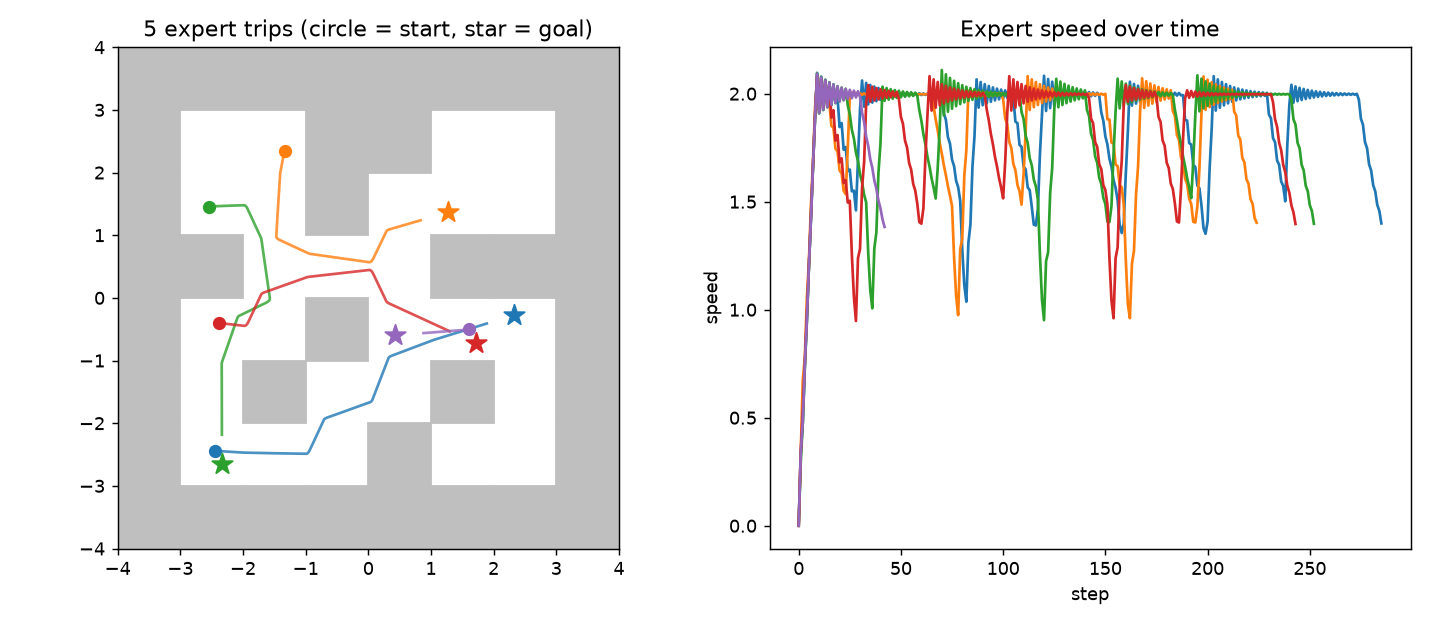
\includegraphics[width=\columnwidth]{expert_trajectories.png}
\caption{Five expert trips through the maze (left) and the speed the controller holds along a trip (right). The
500 training trips cover 359 of the 650 possible start and goal pairs; Section~\ref{sec:generalization} scores
policies separately on the 86 of 200 test trips that use a pair the training data never contained.}
\label{fig:expert}
\end{figure}

\subsection{Evaluation metrics}\label{sec:metrics}
Every policy drives the same $M=200$ test trips, fixed by one random seed. For trip $j$, let
$\text{succ}_j\in\{0,1\}$ record whether the goal was reached, $T_j$ the steps taken, $L_j$ the distance
travelled, $L^*_j$ the expert's distance on the same trip, and let $S$ be the set of successful trips. The four
metrics are
\begin{align}
\text{Success}&=\tfrac{1}{M}\textstyle\sum_j \text{succ}_j,\\
\text{Collision}&=\tfrac{1}{M}\textstyle\sum_j \mathbf{1}[\text{wall contact in trip } j],\\
\text{Efficiency}&=\tfrac{1}{|S|}\textstyle\sum_{j\in S}L^*_j/L_j,\\
\text{Time}&=\tfrac{1}{|S|}\textstyle\sum_{j\in S}T_j .
\end{align}
A wall contact is a MuJoCo contact between the ball and a wall with signed distance at most zero; near contacts
inside MuJoCo's 2 mm margin do not count. The collision metric is a yes or no outcome per trip, so a trip that
scrapes a wall once and a trip that scrapes it ten times count the same. The expert scores 1.0 on efficiency by
construction.

Efficiency and time are averaged over completed trips only, which hides damage in a specific way: a policy that
fails its hardest trips keeps a flattering average on the trips it still finishes. We therefore report a second
efficiency measure over all $M$ trips with a failed trip scored zero,
\begin{equation}
\text{Efficiency}_{\text{all}}=\tfrac{1}{M}\textstyle\sum_j \text{succ}_j\, L^*_j/L_j ,
\label{eq:effall}
\end{equation}
which cannot be inflated this way.

\subsection{Statistical tools}\label{sec:tools}
Three standard tools carry the claims in this report, and each answers a different question about the same
comparison.

A permutation test asks whether a gap between two groups is larger than relabeling the group members at random
would produce. With ten policies on each side there are $\binom{20}{10}=184{,}756$ possible relabelings, and
with five there are $\binom{10}{5}=252$, both few enough to enumerate exactly rather than sample, which makes
the resulting p value exact at the resolution the design allows. When the two groups are matched rather than
independent, the relabeling has to respect the matching: flipping the label inside each pair gives $2^{10}=1{,}024$
assignments at ten seeds and $2^5=32$ at five. The paired version is the more faithful test of this design and
the coarser one, and we report both.

A bootstrap resamples the data with replacement many times and reads an interval off the spread of the resulting
estimates \cite{efron}. Resampling the shared test trips once per draw and applying that same sample to every
dataset keeps the comparison paired, which removes the variation caused by some test trips being harder than
others.

Holm's step down procedure controls the probability of at least one false positive across a family of
comparisons by testing the sorted p values against progressively weaker thresholds \cite{holm}. It is uniformly
more powerful than a plain Bonferroni correction and makes no assumption about independence between the tests.

%=======================================================================
\section{Method}

\subsection{Expert demonstrations}
The expert plans a route over maze cells with breadth first search and steers along it with a two layer
proportional derivative controller. For the next waypoint $w$, position $p$ and velocity $v$, the controller sets
a desired velocity and then a force,
\begin{align}
v^{\text{des}}&=k_p\,(w-p),\quad \text{capped at } \|v^{\text{des}}\|\le v_{\max},\\
a&=\clip\!\big(k_v\,(v^{\text{des}}-v),\,-1,\,1\big),
\end{align}
with $k_p=3$, $k_v=8$ and $v_{\max}=2$, found by grid search and reaching 100\% success on 150 random trips. The
clean dataset holds 500 trips between random start and goal cells, all successful, with 106{,}543 steps in total
and between 15 and 463 steps per trip. We generate the demonstrations ourselves instead of downloading an
existing set, since each flawed driver has to replay the expert's exact trips for the comparison to hold
everything else fixed.

\subsection{Injecting mistakes}
Every corrupted dataset replays the same 500 trips as the clean data, with the same start cell, goal cell and
simulator seed. In the main comparison the same 100 trips, a 20\% share, are handed to the flawed driver for
every error type, so the six datasets differ only in what the flawed driver does. Section~\ref{sec:results} adds
50\% and 100\% versions, nested inside each other, and three versions cut to an equal number of wrong steps. The
trips that stay clean in every dataset are byte identical to the clean data.

The flawed driver really drives the ball through the simulator, so every recorded state is the true result of the
action before it. Editing actions in a finished file would break that link and produce demonstrations no physical
system could have generated. Each mistake was made stronger until it was clearly visible in plots and in wall
contacts, which the expert never produces. Some routes have no corner, or no side corridor on the chosen side,
and those trips stay clean even when selected. Of the 100 flawed trips in the main comparison, the mistake
appears in 84 for the wrong left turn, 89 for the wrong right turn, 85 for the delayed turn, 99 for wall hugging,
96 for missing recovery and 100 for the fast speed. For missing recovery, 1{,}550 recovery steps are left out of
the data. Table~\ref{tab:errors} gives what each flawed driver does and how much of the training data its mistake
touches, and Figure~\ref{fig:mazes} draws five of the six on the maze against the expert's own route.

\begin{table*}[tbp]
\centering\small
\begin{tabular}{@{}>{\raggedright\arraybackslash}p{3.0cm}p{8.6cm}ccc@{}}
\toprule
Error & What the flawed driver does & Wall contact & Extra steps & Error steps\\
\midrule
wrong left turn & once per trip, at a random junction with an open side corridor on the left, drives into it for 25 steps, then plans a new route & 0\% & 31 & 1.9\%\\
wrong right turn & the same, to the right & 0\% & 31 & 2.0\%\\
speed too fast & speed cap $v_{\max}=3$ instead of 2 for the whole trip & 0\% & $-27$ & 11.6\%\\
delayed turn & at every corner keeps going straight for 45 steps, past the corner and into the wall ahead, then turns & 79\% & 91 & 9.2\%\\
wall hugging & aims 0.38 toward a side wall instead of the cell center, leaving a gap of 0.02 & 32\% & 43 & 15.4\%\\
missing recovery & once per trip is pushed off its route (force 0.5 for 25 steps); the slip is recorded, the steps that steer back are left out & 26\% & 12 & 2.2\%\\
\bottomrule
\end{tabular}
\caption{The six error types, at the 20\% corrupted share used in the main comparison. Wall contact and extra
steps describe the flawed trips, against the same trips driven by the expert. Error steps: share of all training
steps where the mistake is active. Speed too slow ($v_{\max}=1$) made 10 of 100 trips time out and is held back.}
\label{tab:errors}
\end{table*}

\begin{figure*}[tbp]
\centering
\begin{subfigure}{0.19\textwidth}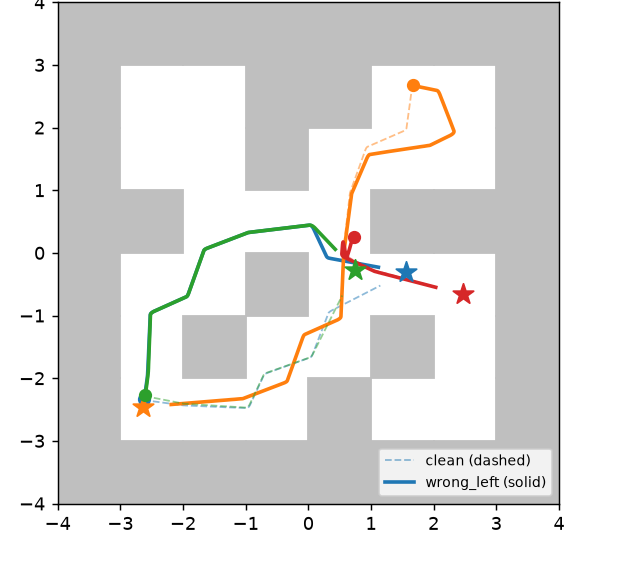
\includegraphics[width=\linewidth]{maze_wrong_left.png}\caption{wrong turn (left)}\end{subfigure}\hfill
\begin{subfigure}{0.19\textwidth}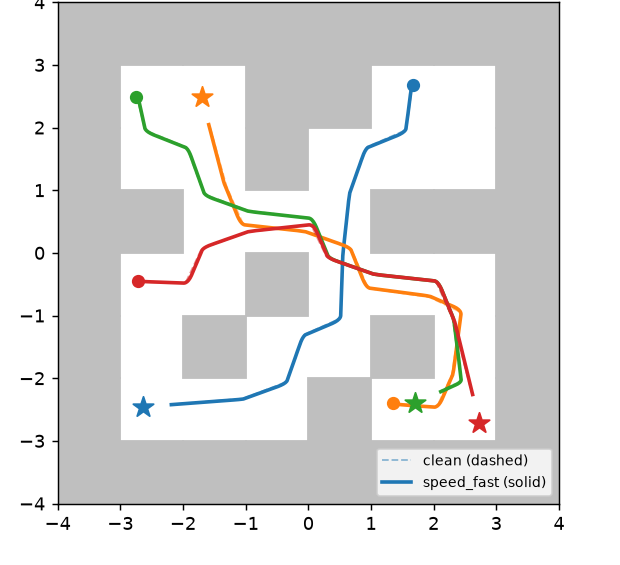
\includegraphics[width=\linewidth]{maze_speed_fast.png}\caption{speed too fast}\end{subfigure}\hfill
\begin{subfigure}{0.19\textwidth}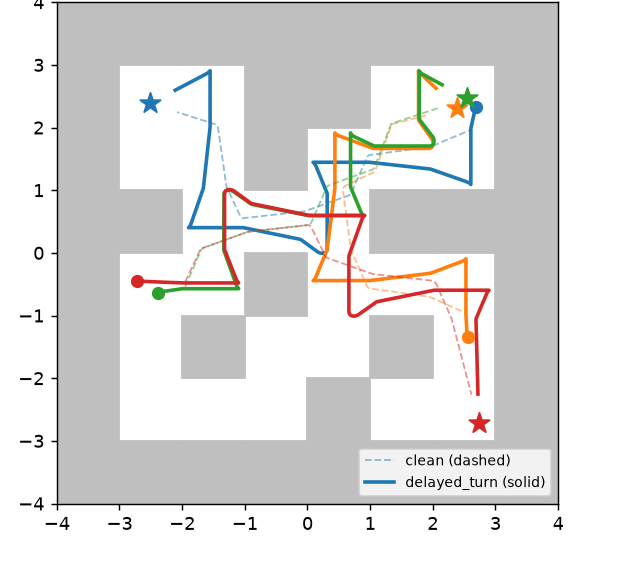
\includegraphics[width=\linewidth]{maze_delayed_turn.png}\caption{delayed turn}\end{subfigure}\hfill
\begin{subfigure}{0.19\textwidth}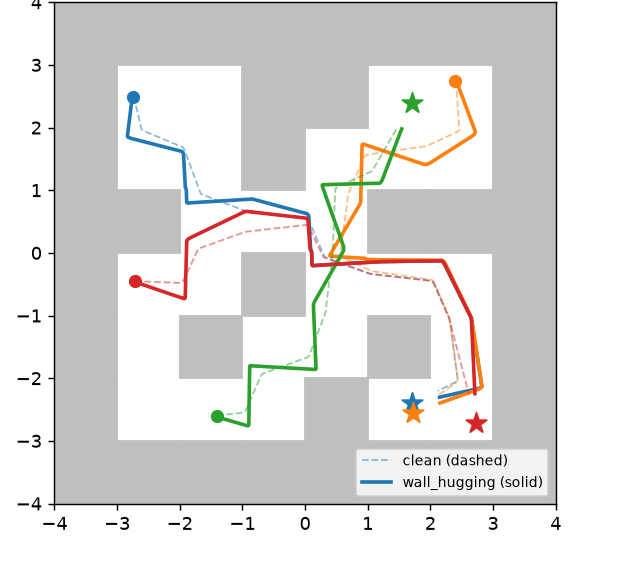
\includegraphics[width=\linewidth]{maze_wall_hugging.png}\caption{wall hugging}\end{subfigure}\hfill
\begin{subfigure}{0.19\textwidth}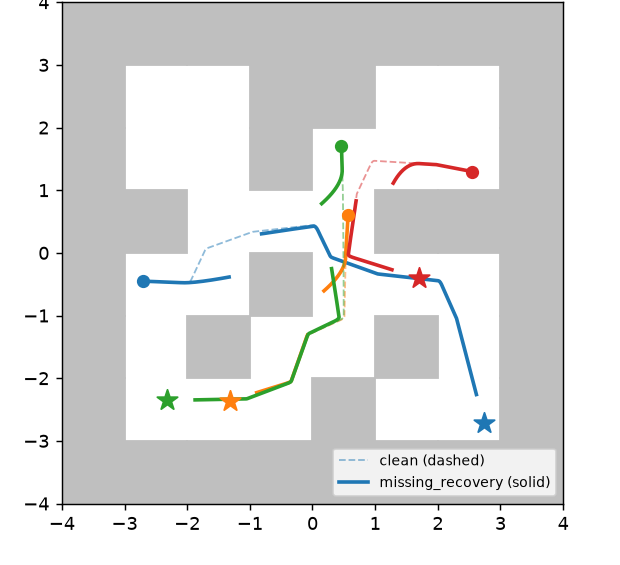
\includegraphics[width=\linewidth]{maze_missing_recovery.png}\caption{missing recovery}\end{subfigure}
\caption{Five of the six error types; the wrong right turn mirrors the left. Each panel shows four corrupted trips
(solid) drawn over the same trips driven by the expert (dashed). Gaps in (e) are the recovery steps left out of
the data.}
\label{fig:mazes}
\end{figure*}

\subsection{Policy and training}\label{sec:training}
The policy is a multilayer perceptron with layer sizes 6, 128, 128, 2, ReLU activations and a final tanh that
keeps the output inside the legal action range. Inputs are standardized with the training mean and standard
deviation, which are stored in the model file. We train with the loss in Equation~\eqref{eq:loss}, Adam
\cite{adam} at learning rate $10^{-3}$, batches of 256 and 120 epochs. A pilot run with 40 epochs gave clean
success of 86\%, 81\% and 93\% across three seeds, against 98\%, 95\% and 94\% with 120 epochs, so we use 120 to
keep the baseline strong and stable. That choice was made by looking at clean success on the same test trips used
for the results, before any corrupted dataset existed, and it is the same for every dataset, so it favors no
error type over another; it remains a limitation of the completed study (Section~\ref{sec:limitations}) rather
than one we were able to remove.

Every dataset is trained with at least five random seeds, where a seed sets the network's initial weights and the
order of minibatches. The study covers 26 datasets, namely clean data, six errors at three corrupted shares,
three errors cut to an equal number of wrong steps, three pairs and one six way mixture, each trained with
seeds 0 to 4. Clean data and the six errors at 20\%, which make up the main comparison, were trained with seeds
5 to 9 as well, for 165 policies in all.

\subsection{Baselines}
The expert driver gives the upper bound and BC on clean data is the reference that every corrupted dataset is
compared against. The midterm's descriptive rule, a difference larger than twice the larger seed standard
deviation, is kept as a quick visual guide in the dose and matched exposure tables and in two figures, but it
is no longer the basis for any claim. Every claim called solid in Section~\ref{sec:results} instead passes the
tests below.

\subsection{Statistical procedure}\label{sec:stats}
Every comparison uses the seeds both sides share, so seed $s$ of one dataset always meets seed $s$ of the other.
For clean BC against the six main errors at 20\% that is ten seeds on each side. Every other dataset has five,
and its comparisons use clean BC's seeds 0 to 4. On those seeds we measure four things, using the tools
described in Section~\ref{sec:tools}.

\subsubsection{Permutation test}
The clean and flawed training runs are pooled and re split into every possible pair of equal groups, holding the
200 test trips fixed. The p value is the share of those splits whose gap is at least as large as the one
observed. Across the six main errors we apply Holm's correction. The number of seeds sets a floor under this
value: at ten against ten the smallest p value is $2/184{,}756\approx0.00001$, or $0.0001$ after correction, and
at five against five it is $2/252\approx0.0079$, or $0.048$ after correction. This test treats the runs as
exchangeable, while the same seed numbers are reused across every dataset, so the runs are matched by seed rather
than fully independent draws; the paired test below does not need that assumption.

\subsubsection{Paired permutation test}
The unpaired test above treats the runs as exchangeable, which the shared seeds argue against, so we run the
matched version of the same idea as a check on it. Seed $s$ of a dataset and seed $s$ of clean BC form a pair,
and the label inside every pair is flipped in all possible ways, giving the share of assignments whose mean
difference is at least as large in size as the observed one. This respects the pairing exactly, at a cost in
resolution. At ten seeds the smallest p value it can return is $2/1{,}024\approx0.002$, or $0.012$ after Holm
correction for six errors, so it can certify a result. At five seeds the floor is $2/32=0.0625$, or $0.375$ after
correction, so it cannot certify anything at the 0.05 level however large the effect. That limit is why the main
comparison was rerun with ten seeds.

\subsubsection{Paired bootstrap interval}
Each of 10{,}000 draws samples the 200 test trip positions once, with replacement, and applies that same sample
to every dataset, keeping the trips paired, then separately samples the training seeds with replacement. The
2.5th and 97.5th percentiles of the resulting differences give a 95\% interval. Its own p value, read from where
the interval sits relative to zero, is reported but not used for the Holm correction, since it answers a
different question than the permutation p value.

\subsubsection{Seed matched interval}
For dataset $X$ and seed $s$ we take the difference between $X$'s seed $s$ policy and clean BC's seed $s$ policy,
giving one matched difference per seed, and compute a classic $t$ interval from them. This check uses the shared
seed numbers directly rather than discarding them, and does not require treating the runs as exchangeable.

Two bars are reported separately for every comparison, since they can disagree. The first asks whether the
bootstrap interval and the seed matched interval both exclude zero. The second asks whether the permutation p
value survives the Holm correction across the six main errors. We call a result solid only when it clears both,
which three of the six main errors do, and all three clear the paired test as well; an error that clears the
intervals alone is reported as such rather than folded in with them.

\subsection{Unseen route generalization check}\label{sec:gen-method}
The 500 training trips cover 359 of the 650 possible ordered start and goal pairs. Of the 200 fixed test trips,
114 use a pair that appears in training and 86 use a pair that never does, though every individual cell appears
in training as both a start and a goal, so an unseen test trip is a new route through a known maze rather than a
new maze. Splitting the test trips on this line and scoring each half separately needs no retraining; it only
reads the start and goal cell already stored in each saved trip.

\subsection{Diagnosis classifier}
The evaluator saves one row per test trip, holding the outcome, the steps taken, the end point, the first wall
contact and the number of contact steps. We reduce each policy to eight numbers computed from these rows: success
rate, collision rate, share of trips that hit the 600 step cap, steps divided by the expert's steps on the same
trips, distance per step, path efficiency on completed trips, mean distance to the goal at the end of failed
trips, and wall contact steps per trip that touched a wall. A logistic regression and a random forest of 300
trees \cite{breiman} each predict the training error from those eight numbers.

Scoring always leaves one seed out: the model trains on the policies of every other seed and predicts the
policies of the held out seed, once for each seed, so a model is never scored on a policy whose seed it trained
on. The six errors at 20\% have ten seeds, which gives 60 policies in the main result; the 50\% and 100\% shares
have five seeds, so seeds 5 to 9 of the pooled run hold only 20\% policies. Clean BC is not one of the six classes
in the main result. Past that result we test two harder questions, namely naming the error at a corrupted share
held out of training entirely, by training on the other two shares with the test seed left out and predicting the
held out share at that seed, and telling a clean policy from a flawed one as a first stage, with the two classes
weighted equally since there are ten clean policies against sixty flawed ones. Two sanity checks close the
analysis: scoring 300 runs with the error labels shuffled, and dropping each input feature in turn.

\subsection{Reproducibility}
The study runs on Python 3.11, PyTorch on a CPU and Gymnasium Robotics 1.4 with MuJoCo, and one policy trains in
about one minute. The demonstration data is fixed by data seed 0. The commands \texttt{corrupt.py --error all},
\texttt{train\_bc.py --data <file> --seed <k>}, \texttt{evaluate.py --expert}, \texttt{stats\_brick9.py} and
\texttt{generalization.py} rebuild every number in this report from the public repository \cite{repo}.

%=======================================================================
\section{Results}\label{sec:results}

The completed study trained and scored all 165 policies. Training loss falls from about 0.15 to about 0.06 over
120 epochs for every dataset. We lead with the three findings that clear both bars of
Section~\ref{sec:stats}, then place the remaining three errors, the dose and matched exposure runs, the pair
interactions, the unseen route check and the diagnosis classifier around them.

\subsection{The three solid findings}
A delayed turn at corners, a missing recovery step and wall hugging are the three main errors whose effect on the
collision rate clears both bars of Section~\ref{sec:stats}: both intervals exclude zero and the unpaired p value
survives the Holm correction (Table~\ref{tab:stats}). All three clear the paired permutation test as well. Each
returns $0.002$, the floor of that test at ten seeds, which means all ten seed differences share a sign and no
relabeling of the pairs gives a larger mean difference; after correction for six comparisons that is $0.012$.

\begin{table*}[tbp]
\centering\small
\begin{tabular}{@{}lccccccccc@{}}
\toprule
& & & & \multicolumn{2}{c}{Unpaired} & \multicolumn{2}{c}{Paired} & Both & Holm\\
\cmidrule(lr){5-6}\cmidrule(lr){7-8}
Error (20\% of trips) & Change & Bootstrap 95\% & Seed 95\% & $p$ & Holm $p$ & $p$ & Holm $p$ & intervals & sig.\\
\midrule
Delayed turn & $\mathbf{+29.75}$ & $[23.85,35.75]$ & $[24.21,35.29]$ & $<0.001$ & $\mathbf{<0.001}$ & $0.002$ & $\mathbf{0.012}$ & yes & yes\\
Missing recovery & $\mathbf{+14.30}$ & $[8.00,20.70]$ & $[9.25,19.35]$ & $<0.001$ & $\mathbf{<0.001}$ & $0.002$ & $\mathbf{0.012}$ & yes & yes\\
Wall hugging & $\mathbf{+10.95}$ & $[4.25,17.75]$ & $[6.07,15.83]$ & $0.001$ & $\mathbf{0.005}$ & $0.002$ & $\mathbf{0.012}$ & yes & yes\\
Speed too fast & $+6.15$ & $[-0.70,13.20]$ & $[-0.87,13.17]$ & $0.072$ & $0.217$ & $0.084$ & $0.252$ & no & no\\
Wrong left turn & $0.00$ & $[-6.50,7.00]$ & $[-7.65,7.65]$ & $1.000$ & $1.000$ & $1.000$ & $1.000$ & no & no\\
Wrong right turn & $-0.15$ & $[-6.70,6.60]$ & $[-7.86,7.56]$ & $0.974$ & $1.000$ & $0.979$ & $1.000$ & no & no\\
\bottomrule
\end{tabular}
\caption{Change in collision rate against clean BC, in points, for the six main errors at a 20\% corrupted share,
ten seeds on each side. The unpaired permutation test reshuffles the twenty policies freely; the paired one flips
the label inside each of the ten seed pairs and bottoms out at $0.002$, or $0.012$ after correction. The last two
columns separate the two bars a result can clear: whether the bootstrap and the seed matched intervals both
exclude zero, and whether the unpaired $p$ survives the Holm correction for six comparisons. Delayed turn,
missing recovery and wall hugging clear both, and the paired test after correction as well.}
\label{tab:stats}
\end{table*}

Ten seeds changed one verdict. At five seeds wall hugging cleared both intervals, at $+9.7$ points, but its
corrected p value was $0.159$, and the paired test could not separate it from the other two: at five seeds all
three sat on that test's floor of $0.0625$, and no corrected paired value could fall below $0.375$. With ten seeds
its corrected p value is $0.005$. The opposite happened to speed too fast, which fell from $+9.1$ points to
$+6.15$ and stays short of every bar. The solid effects shrank a little as the seed count doubled, delayed turn
from $+33.2$ to $+29.75$ and missing recovery from $+15.7$ to $+14.30$, which is common when an estimate rests on
few seeds, and the ranking did not change.

Delayed turn raises wall contact from 29.25\% of trips to 59.00\%, the largest effect in the study by a wide
margin; its ten seeds range from 53.5\% to 63.5\%, all far above the highest clean seed at 35.5\%. It lowers path
efficiency from 0.892 to 0.807 and adds about 26 steps to the average trip, and it lowers success by 4.75 points,
a change both intervals call real but whose corrected p value, 0.051, falls just short. Missing recovery raises
wall contact by 14.30 points and wall hugging by 10.95, while both leave success, path efficiency and time close
to clean. All three effects hold on the 86 of 200 test trips whose start and goal pair the training data never
contained (Section~\ref{sec:generalization}), so none is an artifact of the policy repeating memorized routes.

\subsection{The other three errors at a 20\% share}
Table~\ref{tab:results} gives every metric for all six errors at the 20\% share, and Figure~\ref{fig:results}
shows the collision and success rates with their spread across seeds.

\begin{table*}[tbp]
\centering\small
\begin{tabular}{@{}lccccc@{}}
\toprule
Policy & Success (\%) & Collisions (\%) & Change & Path efficiency & Time to goal\\
\midrule
Expert driver (upper bound) & 100 & 0 & & 1.000 & 211\\
BC, clean & $91.65\pm2.73$ & $29.25\pm6.17$ & & $0.892\pm0.020$ & $249\pm9$\\
\midrule
BC, delayed turn & $86.90\pm4.31$ & $\mathbf{59.00\pm3.44}$ & $\mathbf{+29.75}$ & $0.807\pm0.020$ & $274\pm7$\\
BC, missing recovery & $89.20\pm2.44$ & $\mathbf{43.55\pm4.88}$ & $\mathbf{+14.30}$ & $0.861\pm0.021$ & $252\pm6$\\
BC, wall hugging & $88.60\pm3.61$ & $\mathbf{40.20\pm7.06}$ & $\mathbf{+10.95}$ & $0.873\pm0.021$ & $257\pm8$\\
BC, speed too fast & $91.65\pm2.33$ & $35.40\pm7.97$ & $+6.15$ & $0.899\pm0.027$ & $234\pm9$\\
BC, wrong left turn & $89.10\pm5.97$ & $29.25\pm7.66$ & $0.00$ & $0.862\pm0.020$ & $261\pm7$\\
BC, wrong right turn & $89.60\pm2.98$ & $29.10\pm7.47$ & $-0.15$ & $0.873\pm0.017$ & $258\pm5$\\
\bottomrule
\end{tabular}
\caption{Results on 200 fixed test trips, mean $\pm$ standard deviation over ten seeds, at the 20\% corrupted
share. ``Change'' is the collision rate minus the clean collision rate, in points. A rate over ten policies of 200
trips each is an exact multiple of 0.05 points, so percentages carry two decimals. Bold marks the three errors
that clear both bars of Table~\ref{tab:stats}.}
\label{tab:results}
\end{table*}

\begin{figure}[tbp]
\centering
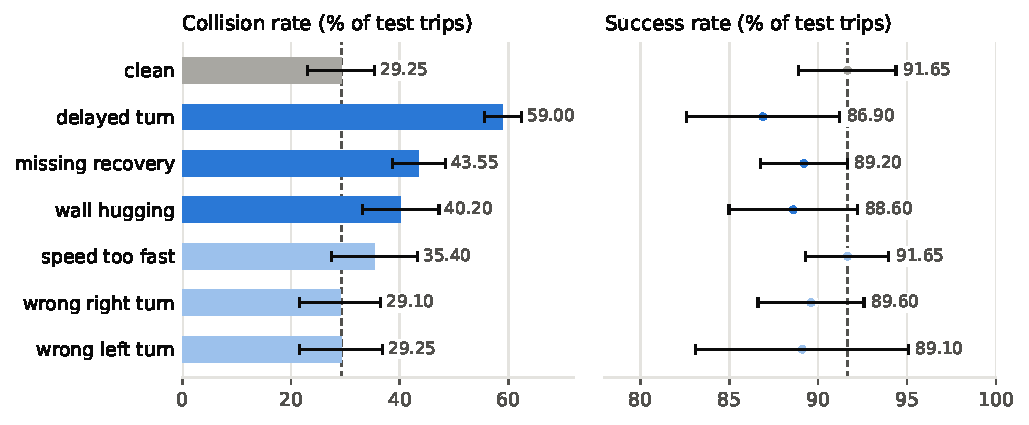
\includegraphics[width=\columnwidth]{results_chart.pdf}
\caption{Collision rate and success rate per dataset over ten seeds; whiskers show one standard deviation and the
dashed line marks the clean baseline. Dark bars mark the three errors that clear both bars of
Table~\ref{tab:stats}, pale bars the three that do not. Drawn from the results file by
\texttt{Reports/make\_chart.py}.}
\label{fig:results}
\end{figure}

BC falls short of the expert even on clean data. Trained on 500 perfect trips, the policy fails 8\% of test
trips, touches a wall on 29\% and takes 18\% more steps than the expert. No wrong label causes this; it is the
compounding error described by Ross and Bagnell \cite{ross2010}. One clean seed is low, at 16\% wall contact
against 22.5\% to 35.5\% for the other nine, and it stays in the results, where it widens the clean spread.

Speed too fast raises collisions by 6.15 points at this share, short of every bar. It makes trips shorter on
average, 234 steps against 249, which fits a policy that learned to drive faster; Section~\ref{sec:dose} shows
this is a working style rather than a mistake once it is the only speed in the data.

Wrong turns show no effect at this share. Both sit within a fifth of a point of clean on collisions, at 0.00 and
$-0.15$, and neither interval in Table~\ref{tab:stats} comes close to excluding zero. Section~\ref{sec:dose}
shows that this null result does not hold at a higher corrupted share.

\subsection{Dose: 20\%, 50\% and 100\% of the trips}\label{sec:dose}
The dose, matched exposure and pair studies in this and the next two subsections each add datasets that have
five seeds, so they compare everything on seeds 0 to 4, clean BC and the six errors at 20\% included. Their 20\%
values are therefore the five seed ones, $+33.2$ for delayed turn rather than the $+29.75$ of
Table~\ref{tab:stats}, and their conclusions rest on five seeds.

\begin{figure*}[tbp]
\centering
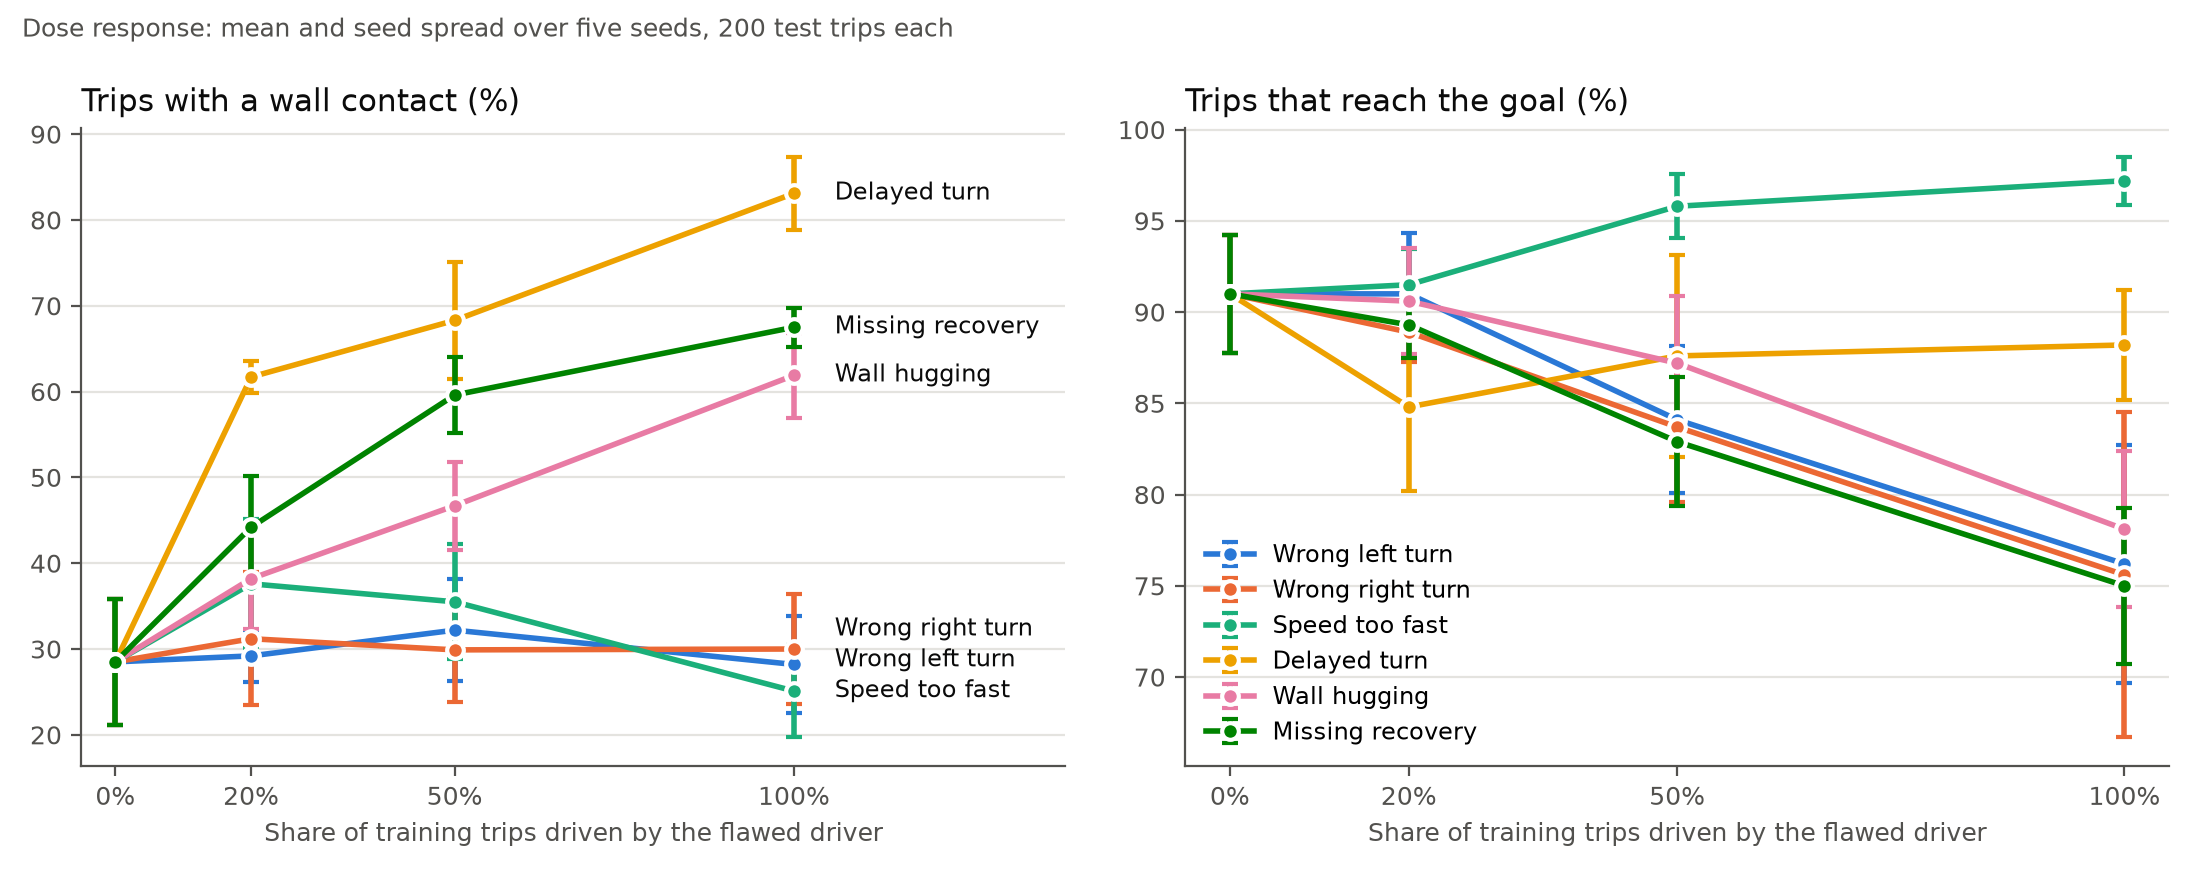
\includegraphics[width=\textwidth]{brick7_dose.png}
\caption{Collision rate and success rate as the corrupted share grows from none of the trips to all of them, seeds
0 to 4 at every share. The point at 0\% is clean BC.}
\label{fig:dose}
\end{figure*}

\begin{table}[tbp]
\centering\small
\begin{tabular}{@{}lcccccc@{}}
\toprule
& \multicolumn{3}{c}{Collisions (\%)} & \multicolumn{3}{c}{Success (\%)}\\
\cmidrule(lr){2-4}\cmidrule(lr){5-7}
Error & 20\% & 50\% & 100\% & 20\% & 50\% & 100\%\\
\midrule
clean data & \multicolumn{3}{c}{$28.5$} & \multicolumn{3}{c}{$91.0$}\\
wrong left turn & $29.2$ & $32.2$ & $28.2$ & $91.0$ & $84.1$ & $\mathbf{76.2}$\\
wrong right turn & $31.2$ & $29.9$ & $30.0$ & $88.9$ & $83.7$ & $75.6$\\
speed too fast & $37.6$ & $35.5$ & $25.1$ & $91.5$ & $95.8$ & $97.2$\\
delayed turn & $61.7$ & $\mathbf{68.3}$ & $\mathbf{83.1}$ & $84.8$ & $87.6$ & $88.2$\\
wall hugging & $38.2$ & $\mathbf{46.7}$ & $\mathbf{61.9}$ & $90.6$ & $87.2$ & $\mathbf{78.1}$\\
missing recovery & $44.2$ & $\mathbf{59.6}$ & $\mathbf{67.5}$ & $89.3$ & $\mathbf{82.9}$ & $\mathbf{75.0}$\\
\bottomrule
\end{tabular}
\caption{Collision and success rate as the corrupted share grows, mean over seeds 0 to 4, so the 20\% column
holds the five seed values rather than those of Table~\ref{tab:results}. Bold marks a difference from clean BC
larger than twice the larger seed standard deviation, the midterm's descriptive rule.}
\label{tab:dose}
\end{table}

Table~\ref{tab:dose} and Figure~\ref{fig:dose} follow each error from a fifth of the trips to all of them.
Delayed turn, missing recovery and wall hugging all get worse as the corrupted share grows, reaching 83\%, 68\%
and 62\% wall contact at 100\%. Wall hugging clears the midterm's rule from 50\% on, and both of its intervals
exclude zero at every share; at 20\% its effect falls short of the correction on these five seeds and clears it
at ten (Table~\ref{tab:stats}).

Wrong turns never raise wall contact at any share, but they do lower success, from about 90\% to about 76\% at
100\% for both turns, and that drop clears both intervals. The failed trips run
out of time about one cell from the goal after travelling about 10 units, so the policy gets lost rather than
hitting walls. The null collision result for wrong turns at 20\% therefore does not mean wrong turns are
harmless, only that this particular outcome does not show the damage at that share.

Speed too fast helps once it is the only speed in the data. At 100\% it gives the highest success of any policy
in the study, 97\%, with the shortest trips at 194 steps and the fewest wall contacts at 25\%. A speed cap of 3.0
is a valid faster driving style on this maze, and it costs collisions only when it is mixed with the normal speed
of 2.0, as it is in the main comparison.

\subsection{The same amount of wrong data for every error}

\begin{figure}[tbp]
\centering
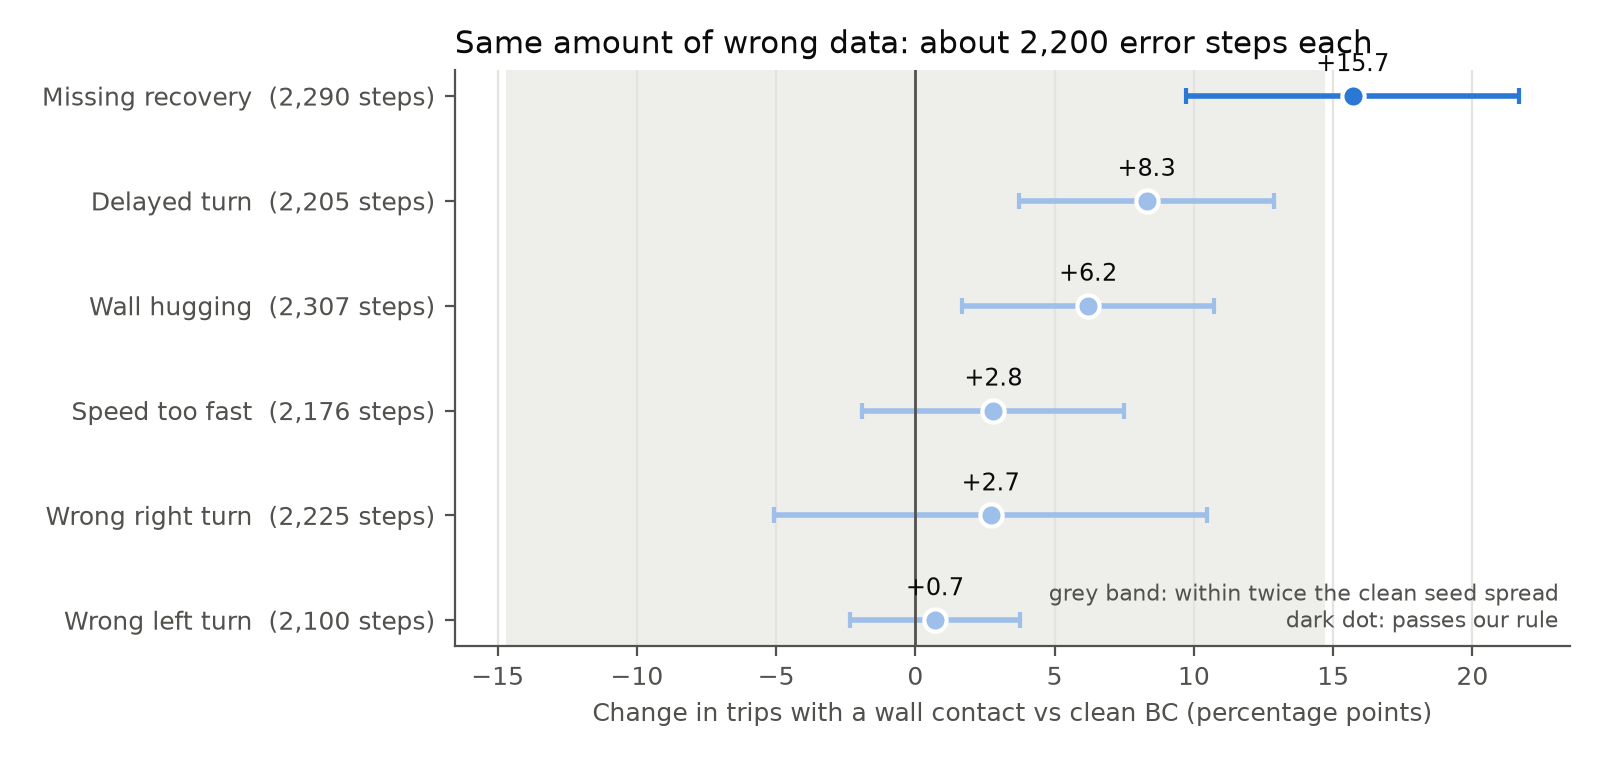
\includegraphics[width=\columnwidth]{brick7_matched.png}
\caption{Change in collision rate against clean BC when every error is cut to about 2{,}200 wrong steps, seeds 0
to 4. The grey band is twice the clean seed spread, the midterm's descriptive rule.}
\label{fig:matched}
\end{figure}

At a 20\% corrupted share the wrong turns and missing recovery carry about 2{,}100 to 2{,}300 wrong steps, while
delayed turn, speed too fast and wall hugging carry 10{,}600 to 17{,}000. Cutting the three larger ones down to
the first 20, 17 and 11 of their usual 100 flawed trips brings all six errors to about 2{,}200 wrong steps each.
Table~\ref{tab:matched} and Figure~\ref{fig:matched} compare them at that matched exposure.

\begin{table}[tbp]
\centering\small
\begin{tabular}{@{}lccc@{}}
\toprule
Error (matched) & Error steps & Collisions (\%) & Change\\
\midrule
clean data & 0 & $28.5$ & \\
wrong left turn & 2{,}100 & $29.2$ & $+0.7$\\
wrong right turn & 2{,}225 & $31.2$ & $+2.7$\\
missing recovery & 2{,}290 & $\mathbf{44.2}$ & $\mathbf{+15.7}$\\
delayed turn (20 trips) & 2{,}205 & $36.8$ & $+8.3$\\
speed too fast (17 trips) & 2{,}176 & $31.3$ & $+2.8$\\
wall hugging (11 trips) & 2{,}307 & $34.7$ & $+6.2$\\
\bottomrule
\end{tabular}
\caption{Collision rate with every error carrying about the same number of wrong steps, seeds 0 to 4.}
\label{tab:matched}
\end{table}

Missing recovery is the only error that clears the midterm's rule at matched exposure, and by this measure it is
the most harmful error in the study, costing about 7 points of wall contact per 1{,}000 wrong steps. Most of the
delayed turn's effect came from its larger volume of wrong data: on the same five seeds, cut to the exposure of a
wrong turn, its effect drops from $+33.2$ to $+8.3$ points. It still ranks second at matched
exposure, ahead of wall hugging, speed too fast and the two wrong turns, though with only five seeds that gap is
itself borderline.

This result sharpens, rather than contradicts, Section~\ref{sec:stats}. Delayed turn earns its solid rank partly
from how often it repeats inside a flawed trip, while missing recovery earns the same rank from a single
occurrence per trip, which is the more surprising of these two and the one Equation~\eqref{eq:bias} does not
explain on its own.

\subsection{Pairs of errors and the mixed dataset}

\begin{figure}[tbp]
\centering
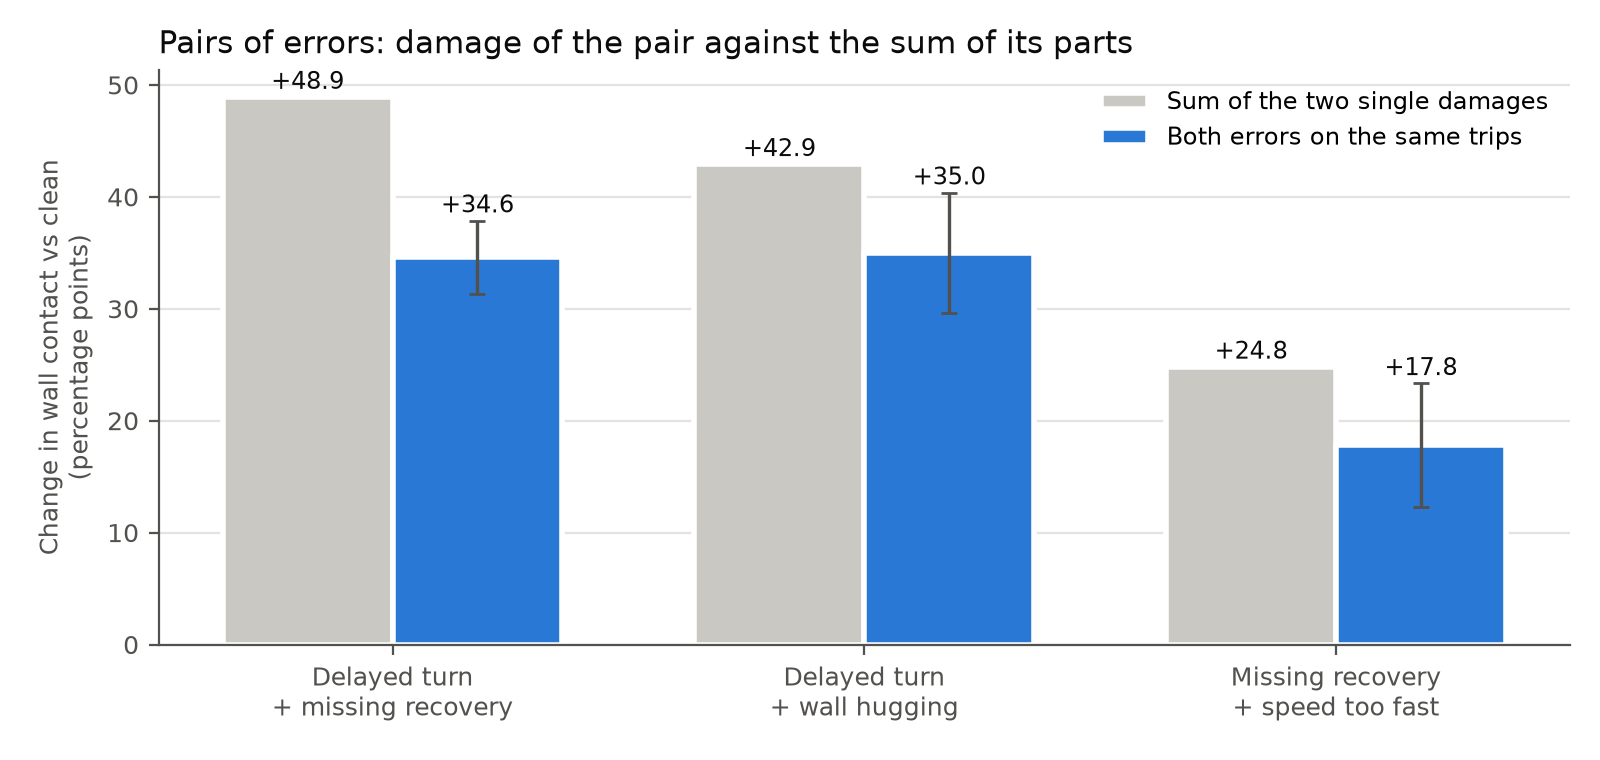
\includegraphics[width=\columnwidth]{brick7_pairs.png}
\caption{Each pair of errors against the sum of the damage its two single errors do on their own. A blue bar
below its grey partner is a pair that hurts less than its parts added together.}
\label{fig:pairs}
\end{figure}

A pair dataset puts both errors on the same 100 flawed trips, so the corrupted share stays at 20\%. The mixed
dataset gives each of the 100 flawed trips one of the six errors in turn. The interaction on collision rate is
$I=m_{A+B}-m_A-m_B+m_{\text{clean}}$, which is zero when the damage adds up, above zero when the pair hurts more
than its parts and below zero when it hurts less. Figure~\ref{fig:pairs} puts each pair against the sum of its
two single errors, and Table~\ref{tab:pairs} gives the interaction with its intervals.

\begin{table}[tbp]
\centering\footnotesize
\begin{tabular}{@{}lccc@{}}
\toprule
Pair or mixture & Coll.\ (\%) & $I$ & 95\% interval\\
\midrule
delayed turn + missing recovery & $63.1$ & $-14.3$ & $[-27.4,-2.7]$\\
delayed turn + wall hugging & $63.5$ & $-7.9$ & $[-17.4,+1.5]$\\
missing recovery + speed too fast & $46.3$ & $-7.0$ & $[-19.1,+4.9]$\\
mixed, less average of six singles & $48.1$ & $+7.8$ & $[+2.0,+13.5]$\\
\bottomrule
\end{tabular}
\caption{Interaction on collision rate on seeds 0 to 4, with the paired bootstrap interval of
Section~\ref{sec:stats}. The seed matched intervals are $[-30.3,+1.7]$, $[-18.2,+2.4]$, $[-21.9,+7.9]$ and $[+2.0,+13.5]$ in the same order. All
three pairs are below additive; the mixed dataset is above the average single error in both intervals, with all
five seeds agreeing.}
\label{tab:pairs}
\end{table}

No pair makes the damage worse than its parts added together. Delayed turn with missing recovery is the clearest
case, below additive in the bootstrap interval though not in the seed interval alone: that pair touches a wall on
63\% of trips, close to delayed turn by itself. Two things push in this direction. Wall contact is a yes or no
outcome per trip, so a trip that already hits a wall from one error cannot count again for the other, and packing
both errors into the same 100 trips leaves fewer total wrong steps, 10{,}802, than the two single datasets hold
between them, 12{,}907.

The mixed dataset hurts more than the average single error dataset, 48.1\% wall contact against 40.3\%, a gap
that excludes zero in both the bootstrap and the seed interval. One reading is that the dose curves in
Section~\ref{sec:dose} are steepest at small corrupted shares, so six errors on about 17 trips each add up to
more damage than one error on 100 trips. That reading is a hypothesis, not yet tested directly.

\subsection{Efficiency counted over all trips}
The path efficiency reported above is measured on completed trips only (Section~\ref{sec:metrics}), so a policy
that fails its hardest trips can look efficient on the trips it keeps. The measure in
Equation~\eqref{eq:effall} scores a failed trip as zero. Clean BC scores 81.75 on that scale over ten seeds, and
80.74 over its first five, which is the baseline for the 100\% column.

\begin{table}[tbp]
\centering\small
\begin{tabular}{@{}lcc@{}}
\toprule
Error & At 20\% (10 seeds) & At 100\% (5 seeds)\\
\midrule
delayed turn & $\mathbf{-11.55}$ & $-21.56$\\
missing recovery & $\mathbf{-4.96}$ & $-21.83$\\
wrong left turn & $-4.95$ & $-19.41$\\
wall hugging & $-4.35$ & $-23.71$\\
wrong right turn & $-3.54$ & $-19.51$\\
speed too fast & $+0.64$ & $+9.78$\\
\bottomrule
\end{tabular}
\caption{Change in efficiency over all 200 trips against clean BC, in points. Bold marks the changes at 20\% that
clear both bars of Section~\ref{sec:stats}.}
\label{tab:effall}
\end{table}

Table~\ref{tab:effall} gives the change against that baseline. At 20\% delayed turn and missing recovery move
this measure by a margin that clears both bars, and delayed turn clears the paired test too (0.012) while missing
recovery does not (0.068). Wall hugging and the wrong left turn clear both intervals but not the correction
(0.100). At 100\% every error except speed too fast costs about 20 points on this
scale, including the two wrong turns, which never raise wall contact yet lose as much ground here as the errors
that do. Speed too fast gains on both efficiency measures, consistent with it being a working faster style rather
than a mistake.

\subsection{Unseen route generalization}\label{sec:generalization}

\begin{table}[tbp]
\centering\footnotesize
\begin{tabular}{@{}lcc@{}}
\toprule
& Seen & Unseen\\
& (114 trips) & (86 trips)\\
\midrule
\multicolumn{3}{@{}l}{\emph{Clean BC, ten seeds}}\\
\quad success & $91.84\%$ & $91.40\%$\\
\quad wall contact & $28.42\%$ & $30.35\%$\\
\midrule
\multicolumn{3}{@{}l}{\emph{Change in wall contact at 20\%, ten seeds}}\\
\quad delayed turn & $+29.30$ & $+30.35$\\
\quad missing recovery & $+15.26$ & $+13.02$\\
\quad wall hugging & $+11.40$ & $+10.35$\\
\quad speed too fast & $+6.58$ & $+5.58$\\
\quad wrong left turn & $+0.44$ & $-0.58$\\
\quad wrong right turn & $-2.11$ & $+2.44$\\
\midrule
\multicolumn{3}{@{}l}{\emph{Change in success at 100\%, five seeds}}\\
\quad wrong left turn & $-15.44$ & $-13.95$\\
\quad wrong right turn & $-17.02$ & $-13.26$\\
\quad speed too fast & $+7.72$ & $+4.19$\\
\bottomrule
\end{tabular}
\caption{Clean BC and the change against it, split by whether the test trip's start and goal pair appeared in
training. Rows at 100\% are compared against clean BC's seeds 0 to 4. The full table for all 26 datasets is in
\texttt{results/generalization.csv} \cite{repo}.}
\label{tab:gen}
\end{table}

Table~\ref{tab:gen} scores the two halves of the split described in Section~\ref{sec:gen-method}, side by side.
Clean BC drives both halves about equally well, 91.84\% against 91.40\% success and 28.42\% against 30.35\% wall
contact, which is what we would expect from a policy that learned to drive the maze rather than to replay
memorized routes.

Every ranking from Table~\ref{tab:stats} holds on the unseen half: delayed turn stays by far the worst, missing
recovery second and wall hugging third, and none of the three solid errors changes sign. The two wrong turns stay
within about two points of zero in both halves. The benefit of the fast speed at 100\% survives too, with success
above clean BC on pairs the training data never contained. This is why this section opens with the three solid
errors rather than treating all six as equally established: they are the only ones that pass both the
statistical tests and the unseen route check. At matched exposure, on five seeds, missing recovery stands out
alone, with delayed turn borderline and wall hugging short of the bars. What this check does not test is a new
maze, since every cell of an unseen pair appears in training as both a start and a goal.

\subsection{Diagnosis: naming the error from the policy's own rollouts}

\begin{figure*}[tbp]
\centering
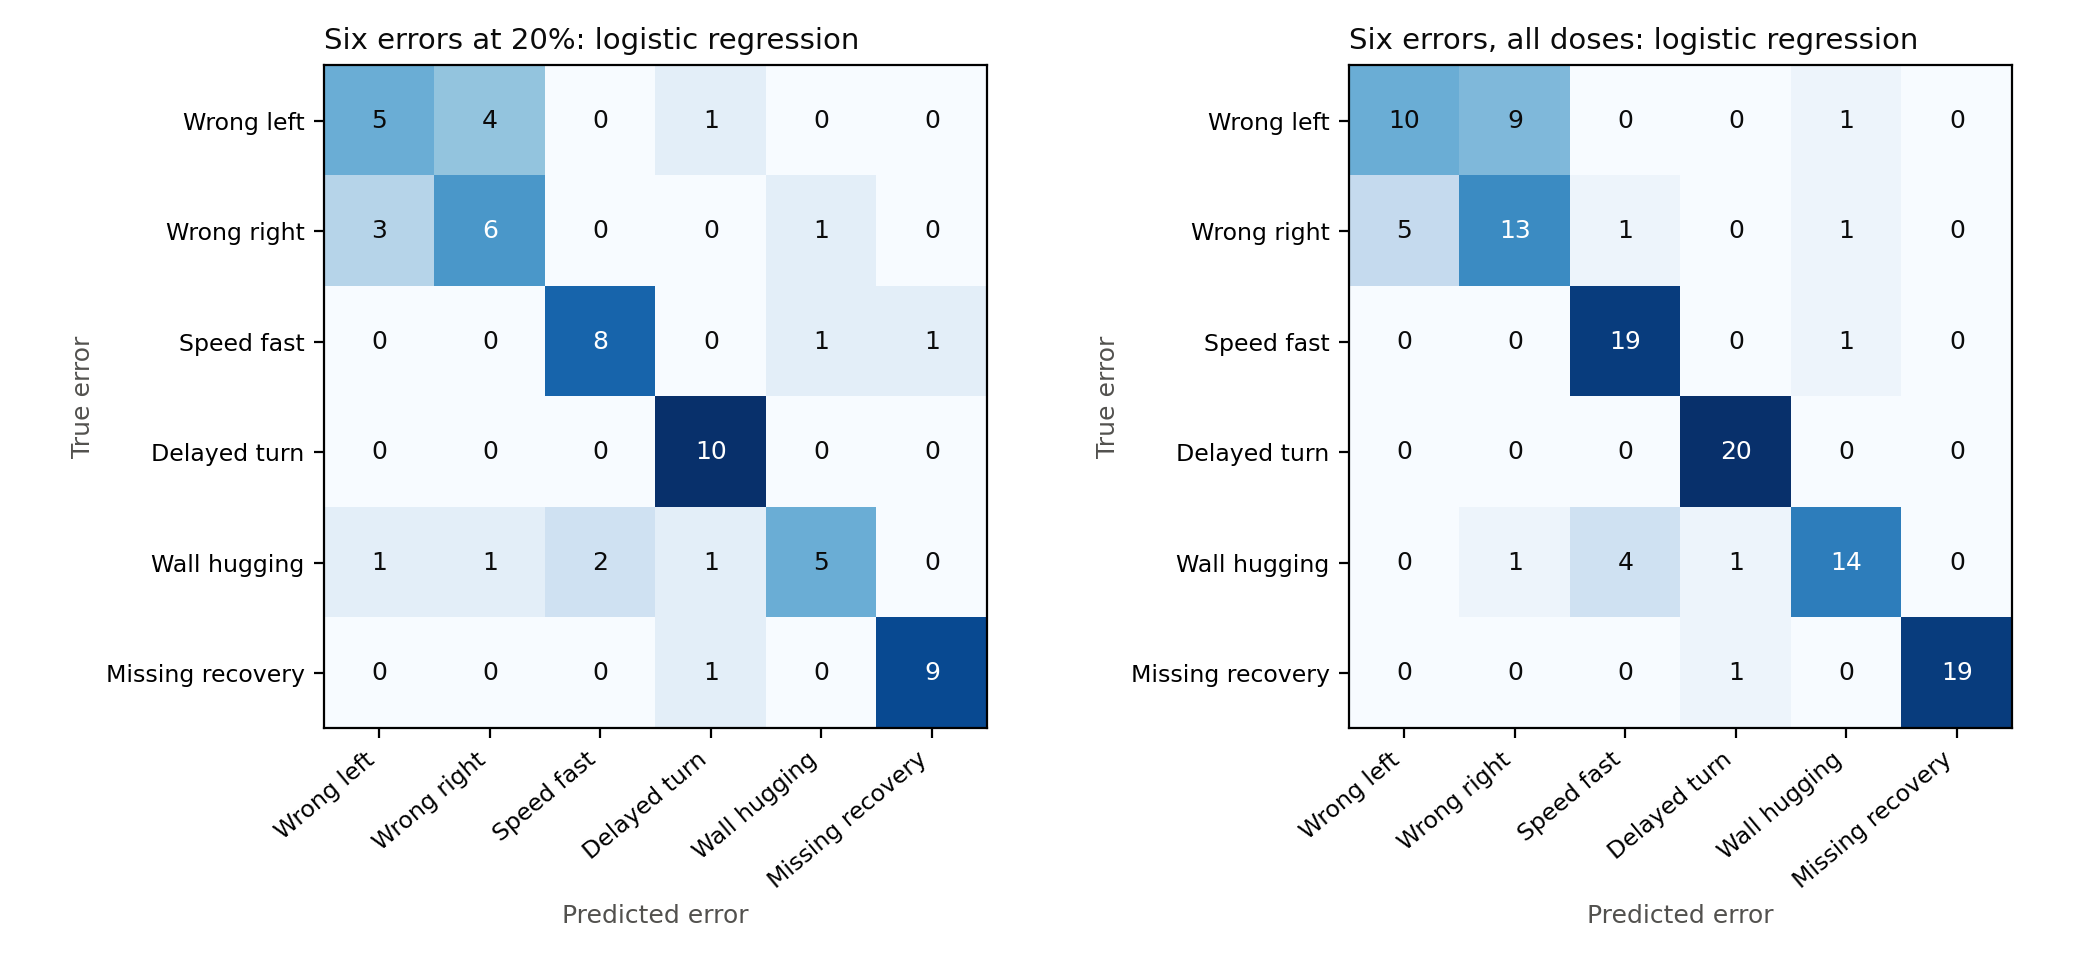
\includegraphics[width=\textwidth]{brick8_confusion.png}
\caption{Confusion matrices for the six class classifier, logistic regression: the main run at a 20\% corrupted
share with ten policies per error (left) and the pooled run across all three shares with twenty per error
(right).}
\label{fig:confusion}
\end{figure*}

\begin{table}[tbp]
\centering\footnotesize
\begin{tabular}{@{}lcccc@{}}
\toprule
Run & Pol. & Chance & Logistic & Forest\\
\midrule
Six errors at 20\% (main) & 60 & 16.7\% & $\mathbf{71.7\%}$ & $56.7\%$\\
Same, wrong turns merged & 60 & & $83.3\%$ & $70.0\%$\\
All three shares (pooled) & 120 & 16.7\% & $79.2\%$ & $72.5\%$\\
Same, wrong turns merged & 120 & & $90.8\%$ & $88.3\%$\\
Clean as a seventh class & 70 & 14.3\% & $55.7\%$ & $54.3\%$\\
\bottomrule
\end{tabular}
\caption{Error type classification accuracy, leave one seed out.}
\label{tab:classify}
\end{table}

Table~\ref{tab:classify} gives the accuracy of every run and Figure~\ref{fig:confusion} shows which errors get
mistaken for which. The main result is 43 of 60 policies, or 71.7\%, against a chance level of 16.7\%. At five
seeds the same run named 25 of 30, or 83.3\%; thirty policies were too few to pin the score down, and the larger
run is the one we report. Delayed turn, missing recovery and speed too fast leave a clear trace: 10, 9 and 8 of
10 policies were named correctly in the main run, and 20, 19 and 19 of 20 when the shares are pooled. The two
wrong turns are mostly confused with each other. Of the five wrong left misses, four were called wrong right, and
of the four wrong right misses, three were called wrong left; counting the two as one class raises the main score
to 83.3\% and the pooled score to 90.8\%. Wall hugging has no single look alike. Five of ten were named
correctly, and the five misses went to four different classes. Its collision rate of 40.2\% sits between speed
too fast at 35.4\% and missing recovery at 43.6\%, and its other seven features all fall inside the range the
other five errors span.

Dropping the collision rate costs 8.3 points, the distance to the goal on failed trips 6.7, speed 5.0 and the
step ratio 5.0, while dropping any of the other four features costs nothing, so no one number carries the result.
With 60 policies the random forest reaches 56.7\%, losing mostly on the wrong turns and wall hugging, and closes
most of the gap once the pooled run gives it twice the data. Shuffling the error labels 300 times and scoring the
same way gives 13.6\% on average and 28.3\% at best, well below the real 71.7\%.

\begin{table}[tbp]
\centering\footnotesize
\begin{tabular}{@{}lcccc@{}}
\toprule
Held out share & Pol. & Logistic & Turns merged & Forest\\
\midrule
20\% & 60 & $58.3\%$ & $65.0\%$ & $58.3\%$\\
50\% & 30 & $96.7\%$ & $100.0\%$ & $83.3\%$\\
100\% & 30 & $66.7\%$ & $83.3\%$ & $63.3\%$\\
All three together & 120 & $\mathbf{70.0\%}$ & $78.3\%$ & $65.8\%$\\
\bottomrule
\end{tabular}
\caption{Accuracy when the model trains on two of the three corrupted shares, with the test seed left out, and is
tested on the third share at that seed. Chance is 16.7\%.}
\label{tab:dose-classify}
\end{table}

Naming the error at a corrupted share never seen in training still works far above chance
(Table~\ref{tab:dose-classify}), at 70.0\% overall and 78.3\% with the wrong turns merged. The 50\% share is the
easy one to hold out, since the classifier only has to interpolate between 20\% and 100\%; the two ends cost 30
to 40 points, since they have to be extrapolated to. The 20\% share is the hardest of the three, and it is the
share where the errors change the policy least.

\begin{table}[tbp]
\centering\footnotesize
\begin{tabular}{@{}lccc@{}}
\toprule
Model & Clean found & Flawed found & Balanced acc.\\
\midrule
Logistic regression & 6 of 10 & $65.0\%$ & $62.5\%$\\
Random forest & 1 of 10 & $96.7\%$ & $53.3\%$\\
\bottomrule
\end{tabular}
\caption{Clean against flawed as a first stage, 10 clean and 60 flawed policies, classes weighted equally. Chance
for balanced accuracy is 50\%.}
\label{tab:stage1}
\end{table}

Telling a clean policy from a flawed one is the weak link (Table~\ref{tab:stage1}). Logistic regression sits a
little above chance, and the forest sits at it by calling nearly every policy flawed. With clean as a seventh
class, only 3 of 10 clean policies are named clean, which fits clean BC and both wrong turns sharing a collision
rate near 29\%. Naming which mistake trained a flawed policy is the part that works; deciding whether there was a
mistake at all is not yet usable on its own.

\subsection{Discussion}
The midterm predicted that navigation mistakes would hurt more than speed mistakes. The completed data does not
support that grouping: the most harmful error, the delayed turn, and the two with the weakest effect at 20\%, the
wrong turns, are all navigation mistakes.

The split that the data does support is consistent with Equation~\eqref{eq:bias}. A delayed turn repeats at every
corner of a flawed trip and always pushes in the direction of travel, so its bias term adds up across many
states. A wrong turn happens once per trip, into a different corridor each time, so its bias term cancels on
average. Wall hugging fits the same account as the delayed turn: a flawed trip aims toward a side wall at every
step, so its bias term points one way across many states, and ten seeds confirm that it transfers. The fast
speed error sits outside this account for a different reason: its bias term is consistent, but
it points toward a policy that is simply faster, which the metrics reward rather than punish once no slower speed
remains in the data to contradict it.

Missing recovery does not fit the account cleanly. It happens once per trip in a random direction, like a wrong
turn, yet Table~\ref{tab:stats} and Table~\ref{tab:matched} both call it solid and the most harmful error per
wrong step in the study. One reading, still a hypothesis and not tested directly here, is that it works through a
different mechanism than the bias term: the data shows the ball drifting off its route but never shows how to get
back, so the policy has no example of recovering once it drifts. That is the opposite of what DART's recovery
labels provide \cite{dart}, and it suggests the quantity that matters for this error is the absence of a
behavior rather than the presence of a wrong action. The super additive interaction of the mixed dataset in
Table~\ref{tab:pairs} is a hypothesis of the same standing, pending the dose curve reading given in
Section~\ref{sec:dose}.

%=======================================================================
\FloatBarrier
\section{Limitations}\label{sec:limitations}

The study uses one maze, PointMaze Medium, and one behavior cloning network, so the results say nothing about
other layouts or other learners. The check in Section~\ref{sec:generalization} is unseen route generalization:
the test trips there are new start and goal pairs inside that same maze, and every cell appears in training as
both a start and a goal, so nothing in this report speaks to a new layout.

The seed count bounds what each comparison can show. The main comparison has ten seeds per side, where the
paired permutation test, which respects the shared seeds, can clear the correction for six errors; its floor
there is 0.012, and the three solid errors reach it. Every other dataset has five seeds, where that test's floor
after correction is 0.375, so it cannot certify anything, and the unpaired test, which assumes the runs are
independent, bottoms out at 0.048. The dose, matched exposure, pair and mixed results therefore rest on the
unpaired test and the two intervals alone. An earlier draft of this report had only five seeds everywhere, and a
review flagged exactly this gap for the main result; ten seeds closed it there and moved wall hugging from
suggestive to established, and the same step for the remaining datasets is the change that would most improve
the rest of the evidence. The diagnosis classifier has ten policies per error at 20\%, so one wrong prediction
moves its main score by 1.7 points, and its accuracy can move by one policy between scikit learn builds.

Every model is the one reached after 120 epochs, with no validation split and no checkpoint selection, and the
epoch count was set by looking at clean data success on the test trips themselves
(Section~\ref{sec:training}). Only 84 of the 100 flawed wrong left trips and 89 of the 100 wrong right trips
contain the mistake, so the effective share of trips carrying those two mistakes is a little below the nominal
20\%. Every condition uses one corrupted dataset built from one draw of which trips to spoil, and the seeds vary
the training run rather than that draw, so these numbers do not say how much a different draw of the same
20\% would move them.

Finally, the established results of this report are the ones called solid in Section~\ref{sec:stats}. The dose
curve reading of the mixed dataset's interaction and the recovery based reading of why missing recovery hurts are
hypotheses that this study did not test directly.

%=======================================================================
\section{Conclusion}

Across 165 trained policies, three of six demonstration mistakes clear every test we apply at ten seeds, a
permutation test with its correction, a seed paired permutation test with the same correction, a paired
bootstrap interval and a seed matched interval, and continue to hold on maze routes the training data never
contained: a delayed turn that repeats at every corner, a missing recovery step that removes the only examples
of returning to the route, and wall hugging that leans toward a wall for the length of a trip. The other three
leave no collision effect at the main corrupted share: the wrong turns are dose dependent and cost success only
once most trips carry them, and the fast speed is beneficial on its own. No pair of mistakes hurts more than the
sum of its parts, while spreading all six across one dataset does. A classifier that sees only a policy's own
test rollouts, never its training data, names which of six mistakes trained it well above chance and keeps most
of that accuracy at a corruption strength it never trained on, though it cannot yet say whether a policy was
trained on flawed data at all, and doubling its data showed its first estimate had been optimistic.

For a practitioner holding a limited cleaning budget, the ranking here points at demonstrations that turn late,
demonstrations with their recoveries missing and demonstrations that hug a wall, and suggests that an occasional
wrong corridor can be left alone at a low corrupted share. What remains open is listed in
Section~\ref{sec:limitations} rather than attempted here: ten seeds for the dose, pair and matched datasets,
repeating the three solid findings with an independent draw of which trips are spoiled, testing a second maze
layout, and adding a validation split to any future training run on this codebase. None of these change what
this report can already say about the three findings it leads with. At ten seeds, a delayed turn, a missing
recovery step and wall hugging are the three demonstration mistakes that this maze and this behavior cloning
policy cannot absorb.

\section*{Contributions}
Abhishek Tyagi led the method, the statistical testing, the generalization check, the diagnosis classifier and
this report. Nishad Gupta ran the training sweeps across datasets and seeds and built the dose and matched
exposure figures. Richard Li built the rollout features behind the diagnosis classifier and contributed to the
related work review and the project's presentation materials. Code, data and every number in this report are
public \cite{repo}.

%=======================================================================
\begin{thebibliography}{99}
\bibitem{pomerleau} D. A. Pomerleau, ``ALVINN: An autonomous land vehicle in a neural network,'' in \emph{NeurIPS}, 1989.
\bibitem{ross2010} S. Ross and J. A. Bagnell, ``Efficient reductions for imitation learning,'' in \emph{AISTATS}, 2010.
\bibitem{dagger} S. Ross, G. Gordon and J. A. Bagnell, ``A reduction of imitation learning and structured prediction to no regret online learning,'' in \emph{AISTATS}, 2011.
\bibitem{dart} M. Laskey, J. Lee, R. Fox, A. Dragan and K. Goldberg, ``DART: Noise injection for robust imitation learning,'' in \emph{CoRL}, 2017.
\bibitem{robomimic} A. Mandlekar et al., ``What matters in learning from offline human demonstrations for robot manipulation,'' in \emph{CoRL}, 2021.
\bibitem{belkhale} S. Belkhale, Y. Cui and D. Sadigh, ``Data quality in imitation learning,'' in \emph{NeurIPS}, 2023.
\bibitem{wu2019} Y. Wu et al., ``Imitation learning from imperfect demonstration,'' in \emph{ICML}, 2019.
\bibitem{sasaki} F. Sasaki and R. Yamashina, ``Behavioral cloning from noisy demonstrations,'' in \emph{ICLR}, 2021.
\bibitem{trex} D. S. Brown, W. Goo, P. Nagarajan and S. Niekum, ``Extrapolating beyond suboptimal demonstrations via inverse reinforcement learning from observations,'' in \emph{ICML}, 2019.
\bibitem{natarajan} N. Natarajan, I. S. Dhillon, P. Ravikumar and A. Tewari, ``Learning with noisy labels,'' in \emph{NeurIPS}, 2013.
\bibitem{hendrycks} D. Hendrycks and T. Dietterich, ``Benchmarking neural network robustness to common corruptions and perturbations,'' in \emph{ICLR}, 2019.
\bibitem{florence} P. Florence et al., ``Implicit behavioral cloning,'' in \emph{CoRL}, 2021.
\bibitem{d4rl} J. Fu, A. Kumar, O. Nachum, G. Tucker and S. Levine, ``D4RL: Datasets for deep data driven reinforcement learning,'' arXiv:2004.07219, 2020.
\bibitem{gymrobotics} Farama Foundation, ``Gymnasium Robotics: Point Maze,'' robotics.farama.org, 2024.
\bibitem{repo} A. Tyagi, N. Gupta and R. Li, ``ImitationLearning\_ErrorStudy,'' GitHub repository, 2026. \url{https://github.com/AbhishekTyagi404/ImitationLearning_ErrorStudy}
\bibitem{adam} D. P. Kingma and J. Ba, ``Adam: A method for stochastic optimization,'' in \emph{ICLR}, 2015.
\bibitem{holm} S. Holm, ``A simple sequentially rejective multiple test procedure,'' \emph{Scandinavian Journal of Statistics}, vol. 6, no. 2, 1979.
\bibitem{efron} B. Efron and R. Tibshirani, \emph{An Introduction to the Bootstrap}. Chapman and Hall/CRC, 1993.
\bibitem{breiman} L. Breiman, ``Random forests,'' \emph{Machine Learning}, vol. 45, no. 1, 2001.
\end{thebibliography}

\end{document}
